\section[Electron waves in crystals]{\hyperlink{toc}{Electron waves in crystals}}

Multiplicity: some families of lattice planes have the same spacing, and thus would in indistinguishable in an XRD experiment.

\begin{figure}
  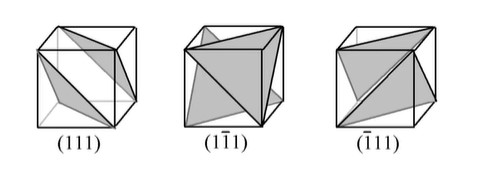
\includegraphics[width=0.75\linewidth]{Images/111 class.jpg}
  \caption{111}
  \label{fig:111}
\end{figure}

ex: {111} signifies all (111) (1$\bar{1}$1) and ($\bar{1}$11) in the so called '111' class. They all diffract with the same angle and thus the line will have a stronger intensity reading compared to other classes without the negative miller indices.

Most common basis structure is sodium chloride NaCl and zinc blende ZnS.

- you can use pattern in XRD or neutron scattering data (i.e. odd peaks (h+k+l=odd) are big and even are small) can tell you which basis it is from.

\textbf{Refresher of Brillouin Zones}

\begin{figure}
  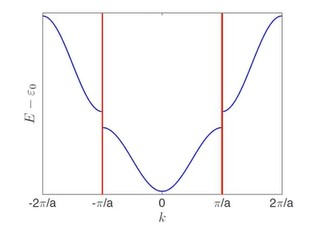
\includegraphics[width=0.75\linewidth]{Images/BrillouinZone.jpg}
  \caption{BZ}
  \label{fig:BZ}
\end{figure}

- You can perform Wigner-Seitz (closest lines drawn, then half way points draw perpendicular lines/planes) method to find 1st,2nd,3rd, etc Brillouin Zones on a lattice.
- first is for the reciprocal lattice point G=0.

\begin{figure}
  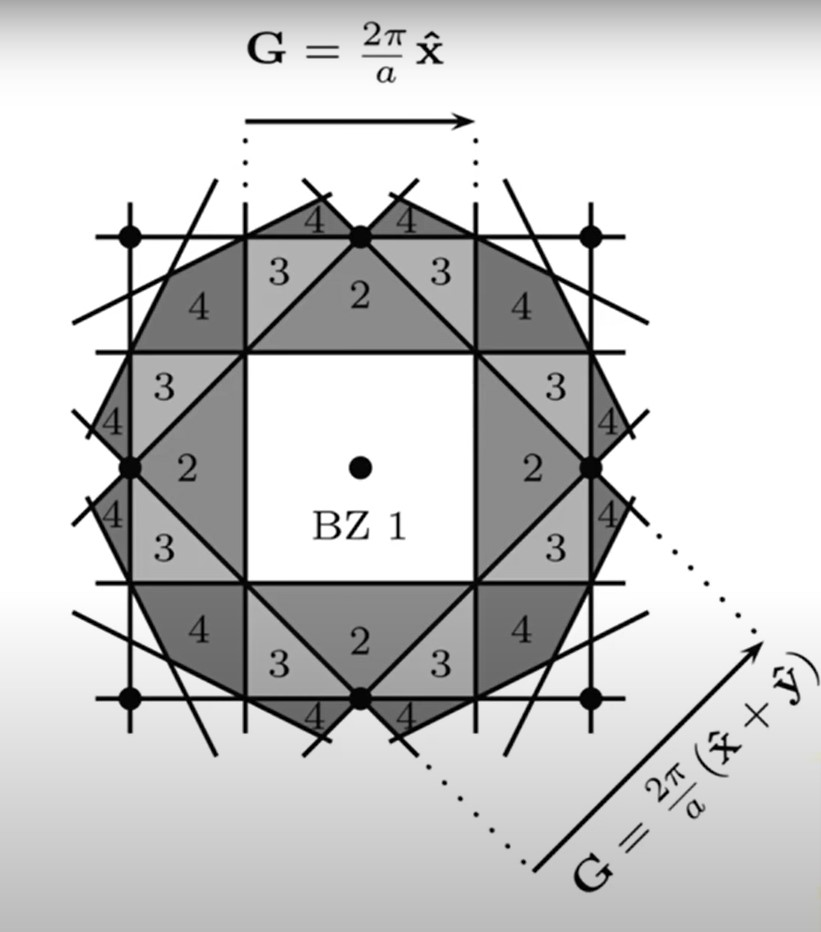
\includegraphics[width=0.75\linewidth]{Images/Bzones.jpg}
  \caption{zones}
  \label{fig:zones}
\end{figure}

- each Brillouin zone has the same area

\textbf{Band Structure in 3D}
- labelling convention to indicate points of symmetry in the Brillouin Zone. Allows us to show structure on a 2D graph.
\begin{itemize}
    \item $\Gamma$ point is the where for k=0
    \item X points at (0, 2$\pi$/a, 0)
    \item L point
    \item $\Sigma$ point
    \item $\Lambda$ point 
    \item W point 
\end{itemize}
 

\textbf{Correspondence} ==> if we start with a FCC lattice in REAL space, then RECIPROCAL lattice will be the BCC lattice.

$\therefore$

1st Brillouin Zone of an FCC lattice  = same shape as Wigner Seitz cell of a BCC lattice.

1st Brillouin Zone of a BCC lattice = same shape as Wigner Seitz cell of an FCC lattice.


- Electron and Phonon Structure can be related to the important points of the Brillouin Zone.



\textbf{Nearly-Free electron model}

- Drude and Sommerfeld models assume free electrons.
- Here we instead impose the crystal structure on a gas of free electrons (and get bands).


\[ H_0 = \frac{p^2}{2m} \]

\[E_0(k) = \frac{\hbar^2k^2}{2m} \]

- Perturbation Theory allows you to find complicated Hamiltonian solutions if we find a known similar system with solution and say there is an additional small perturbation.

 \textbf{Bloch's Theorem}
 - perturbation theory only helps if period potential is weak. 
 - Felix Bloch studied periodic potential Schrodinger equation solutions. 
 - He showed in 1928 that particles in a periodic potential will behave just like free particles except that it is their crystal momentum that is conserved in collisions rather than regular linear momentum.
 
 \begin{figure}
  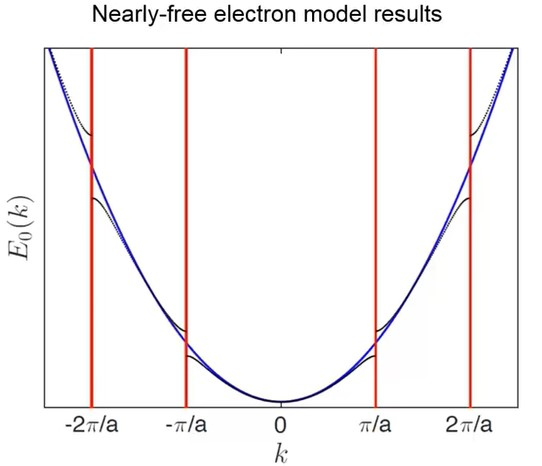
\includegraphics[width=0.75\linewidth]{Images/NearlyFree.jpg}
  \caption{nearly}
  \label{fig:nearly}
\end{figure}
 
 
 Bloch's Theorem is that a particle in a periodic potential has eigenstates of the form:
 
 \begin{tcolorbox}[enhanced,attach boxed title to top center={yshift=-3mm,yshifttext=-1mm},
  colback=blue!5!white,colframe=blue!75!black,colbacktitle=red!80!black,
  title=Bloch's Theorem,fonttitle=\bfseries,
  boxed title style={size=small,colframe=red!50!black} ]
  \begin{equation}
      \psi_\textbf{k}^\alpha (\textbf{r}) = e^{i\textbf{k}\cdot \textbf{r}}u_\textbf{k}^\alpha (\textbf{r}) 
  \end{equation}
\end{tcolorbox}

where \textbf{k} can be chosen to be within the first Brillouin zone, and the function $u_\textbf{k}^\alpha (\textbf{r})$ is a periodic function with period equal to the lattive spacing, which depends on a band index $\alpha$ and on \textbf{k}.

\textbf{- electron motion in crystals is similar to a plane waves! BLOCH WAVES! even if the electrons are strongly bound by the crystal.}
